\documentclass[a4paper]{article}

\usepackage{amsmath, amssymb}
\usepackage{enumitem}
\usepackage{multicol}
\usepackage{parskip}
\usepackage{tikz}
\usepackage{changepage}
\usepackage{tabularray}
\usepackage[T1]{fontenc}
\usepackage[utf8]{inputenc}
\usepackage{mathtools}
\usepackage[a4paper,
            bindingoffset=0in,
            left=0.1in,
            right=0in,
            top=0.1in,
            bottom=0.1in,
            footskip=0.25in]{geometry}
\pagenumbering{gobble}
\usetikzlibrary{shapes.geometric, arrows}
\tikzstyle{arrow} = [thick,->,>=stealth]
\tikzstyle{node} = [ellipse, minimum height=0.5cm,text centered, draw=black, fill=blue!20]

\newcommand{\resetsize}{\small}

\setlist{nosep}
\setlength{\parindent}{0em}
\setlength{\itemindent}{0em}
\setlength{\leftmargini}{0em}

\begin{document}
\begin{multicols*}{2}
    \resetsize
    \subsection*{Terms}
    \setlength{\leftmargini}{7em}
    \begin{itemize}
        \item[OS] provides the environment within which programs are executed
        \item Provides \emph{services} for programs
        \item Provides \emph{interfaces} for users
        \item Collection of \emph{components} and their interconnections
        \item[Parallelism] \(> 1\) task being performed simultaneously \\
            (one process may be waiting on another)
        \item[Concurrency] multiple tasks making progress at one time \\
            (nobody is waiting)
        \item[Throughput] number of processes completed in a unit of time
        \item[Turnaround] from time of submission to completion, \\
            INCLUDING wait time
        \item[Wait Time] time spent in waiting/ready queue, NOT including I/O queue / time
        \item[Response Time] time from submission to time when `first' usable data/output produced
        \item[TLB] Translation Lookaside Buffer
        \item[MMU] Memory Management Unit
        \item[RMS] Rate Monotonic Scheduling
        \item[EDF] Earliest Deadline First
        \item[PTBR] Page Table Base Register (pointer to page table in memory)
    \end{itemize}

    \subsubsection*{Parameter Passing}
    \setlength{\leftmargini}{2em}
    \begin{enumerate}
        \item Pass paramater via registers
        \item Save parameters in block/table (memory), pass via registers the
              address of the block
        \item Placed onto the stack
    \end{enumerate}
    \subsubsection*{System Calls}
    Several basic `types'
    \begin{enumerate}
        \item Process Control \tiny{end, abort, load create process \dots} \resetsize
        \item File Management \tiny{create, delete, open files, \dots} \resetsize
        \item Device Management \tiny{request, write to device, \dots} \resetsize
        \item Info Management \tiny{get process attr, set sys data} \resetsize
        \item Communication \tiny{create, delete, send, receive messages} \resetsize
        \item Protection \tiny{prevent read, allow modification by owner, \dots} \resetsize
    \end{enumerate}

    \subsubsection*{Process}
    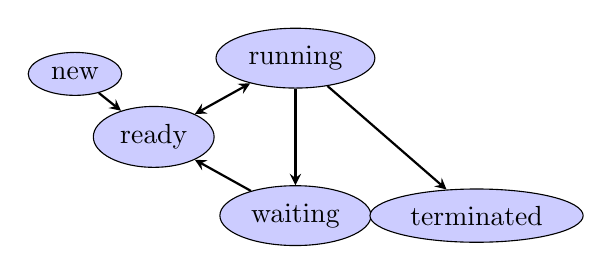
\begin{tikzpicture}[node distance=0.8cm]
        \node (start) [node] {new};
        \node (ready) [node, below of=start, xshift=1cm] {ready};
        \node (running) [node, right of=ready, xshift=1cm, yshift=1cm] {running};
        \node (waiting) [node, right of=ready, xshift=1cm, yshift=-1cm] {waiting};
        \node (terminated) [node, right of=waiting, xshift=1.5cm] {terminated};
        \draw [arrow] (start) -- (ready);
        \draw [arrow, <->] (ready) -- (running);
        \draw [arrow] (running) -- (waiting);
        \draw [arrow] (running) -- (terminated);
        \draw [arrow] (waiting) -- (ready);
    \end{tikzpicture}


    \begin{description}
        \item[New] being created
        \item[Running] being executed
        \item[Waiting] for some event
        \item[Ready] Waiting to be assigned to a processor
        \item[Terminated] Finished execution
    \end{description}


    \begin{tabular}{|c|}
        \hline
        State               \\
        \hline
        Program Counter     \\
        \hline
        CPU Registers       \\
        \hline
        CPU Scheduling Info \\
        \hline
        Mem Mgmt Info       \\
        \hline
        Accounting Info     \\
        \hline
        I/O Status          \\
        \hline
    \end{tabular}
    \\
    Two processes are \emph{independent} if the write set of each is disjoint
    from both the read and write sets of the other.
    % \columnbreak
    \subsection*{Threads}
    \subsubsection*{Many-to-one} All user threads map to a single kernel thread \\
    If a user thread makes a block system call, the entire process (made up of
    multiple user threads) will block Because only 1 thread can access the
    kernel at any one time, multiple threads are unable to run concurrently on a
    multicore computer

    \subsubsection*{One-to-one} Each user thread is mapped to a unique kernel thread \\
    The creation of a user thread requires (considerable) overhead to create a
    kernel thread. If a user thread is idle (perhaps waiting on another thread
    to finish), then the kernel thread with which the user thread is associated
    is needlessly consuming kernel space resources When one thread is blocked
    (user or kernel thread), the other threads can continue. Concurrency is
    enabled

    \subsubsection*{Many-to-many} Many user threads are mapped to a \(\leq \#\)
    kernel threads At the user level, multiple threads are created, and it is up
    to the OS to schedule/orchestrate/map each of them to a kernel thread

    With \(m\) threads with \(n\) instructions each: \[\frac{(mn)!}{(n!)^m}
        \text{ possible histories}\]

    \subsection*{Critical Section Problem}

    \begin{description}
        \item[Mutual Exclusion] If a process is executing its critical section, no others can be executing theirs
        \item[Progress] If no process is executing its critical section, AND
            some process wants to enter its, only those processes NOT executing can
            decide who enters
        \item[Bounded Waiting] There must be a limit on the number of times another process is allowed to enter its critical section after a process has made a request to enter its critical section (i.e., no starvation).
    \end{description}

    \subsubsection*{Semaphores}
    \begin{itemize}
        \item Must be careful NOT to omit an inc/dec in code.
        \item Global, thus must know how entire program works to use them
        \item Can't infer which waiting process will run next
    \end{itemize}
    \subsubsection*{Monitors}
    \begin{description}
        \item[SC] The signaler continues, and the signaled executes at some later time
        \item[SW] The signaler waits until some later time and the signaled executes immediately
    \end{description}
    A monitor follows one, but not both.

    \includegraphics[width=\columnwidth]{scheduling.png}

    \subsection*{Scheduling}
    \begin{multicols*}{2}
        \begin{description}
            \item[FCFS] First Come First Serve
            \item[SJF] Shortest Job First
            \item[Priority] Highest priority first
        \end{description}
        \begin{center}
            \includegraphics[width=\columnwidth]{result.png}
            Priority
        \end{center}
        \columnbreak
        \begin{tabular}{|c|c|c|}
            \hline
            PID & ms & Priority \\
            P1  & 24 & 1        \\
            P2  & 16 & 3        \\
            P3  & 2  & 5        \\
            P4  & 4  & 2        \\
            P5  & 3  & 4        \\
            \hline
        \end{tabular}
    \end{multicols*}
    May encounter issues like starvation / aging. Hence\dots

    \subsubsection*{Round Robin}
    \begin{itemize}
        \item Circular queue
        \item Time quantum
        \item Each process has a given burst time
    \end{itemize}
\end{multicols*}

\newpage

\begin{multicols*}{2}
    \subsection*{Real-time scheduling}
    \begin{description}
        \item[Periodic] occuring at a constant interval / period (p)
        \item[Process time] time needed to burst (t)
        \item[Deadline] time the process must be completed by (d)
    \end{description}

    If a requesting process does not `satisfy' \(0 \leq t \leq d \leq p\), the
    scheduler should reject the process.

    Suppose two processes:
    \begin{description}
        \item[Process 1]  p:50ms, t:20ms, d:1/period
        \item[Process 2]  p:100ms, t:35ms, d:1/period
    \end{description}
    \begin{multicols*}{3}
        Can the CPU process both?
        \columnbreak \\
        \textbf{Utilization (t/p)}
        \begin{align*}
            P1: & 20/50  & = 0.4  \\
            P2: & 35/100 & = 0.35 \\
                &        & 0.75
        \end{align*}
        \columnbreak \\
        Assuming no other process runs, we should be able to service both.
    \end{multicols*}

    \begin{description}
        \item[RMS] Upon entering, a process is assigned a priority inversely
            proportional to its period. (i.e., the shorter the period, the
            higher the priority). P2 would be broken up into two chunks (30 / 5)
            at t=50.
        \item[EDF] Upon entering, a process is assigned a priority inversely
            proportional to its deadline. (i.e., the sooner the deadline, the higher
            the priority).
    \end{description}

    By design, real-time CPU scheduling does not permit a process that has
    already met its period deadline to start a second time in the same period.

    \subsubsection*{Pipeline Stages}
    \begin{multicols*}{2}
        \setlength{\leftmargini}{1em}
        \begin{itemize}
            \item (F)etch
            \item (D)ecode
            \item (E)xecute
            \item (W)rite (B)ack
        \end{itemize}
        \columnbreak
        \begin{tabular}{|c|}
            \hline
            Hard Drive \\
            Memory     \\
            L2 Cache   \\
            L1 Cache   \\
            Registers  \\
            ALU        \\
            \hline
        \end{tabular}
    \end{multicols*}

    \subsection*{Memory Allocation}
    \begin{description}
        \item[Best Fit] Fit into a hole such that resulting left-over hole is
            size minimized (ideally 0)
        \item[First Fit] Fit into first hole (most often reading from bottom
            addresses to higher) that can accomodate the process
        \item[Worst Fit] Fit into largest hole, resulting in left-over hole
            whose size is maximized
    \end{description}

    \subsubsection*{Segmentation}
    Logical Address \(->\) <segment num, offset>
    \begin{equation*}
        \text{Logical Address} -> \begin{cases}
            \text{Segment Number, offset} \\
            S, D
        \end{cases}
    \end{equation*}
    \begin{multicols*}{2}
        S is the index into the table which identifies a row containing limit and base value.
        In the example table, <3, 200>, <3, 60000> would result in address errors
        \columnbreak
        \begin{center}
            Segment Table \\
            \begin{tabular}{c|c}
                limit & base \\
                1400  & 2500 \\
                2600  & 3500 \\
                17000 & 1800
            \end{tabular}
        \end{center}
    \end{multicols*}
    \subsubsection*{Fragmentation}
    \begin{description}
        \item[External] occurs when unused space is non-contiguous
        \item[Internal] refers to the unused space within a frame / page
    \end{description}

    \subsection*{Paging}
    A page size is a power of 2, usually between 512 bytes and 1 GB.
    \begin{multicols*}{2}
        \begin{minipage}{0.5\columnwidth}
            \begin{tblr}{
                    colspec = {c|c|},
                    row{1-4} = {red!5},
                    row{5-8} = {blue!5},
                    row{9-12} = {black!5},
                    row{13-16} = {yellow!5},
                    cell{2}{2} = {orange},
                    cell{6}{2} = {blue},
                    cell{15}{2} = {yellow},
                }
                \cline{2-3} \\
                1 byte & \cline{2-3} \\
                \cline{2-3} \\
                \cline{2-3} \\
                \cline{2-3} \\
                \cline{2-3} \\
                \cline{2-3} \\
                \cline{2-3} \\
                \cline{2-3} \\
                \cline{2-3} \\
                \cline{2-3} \\
                \cline{2-3} \\
                \cline{2-3} \\
                \cline{2-3} \\
                \cline{2-3} \\
                \cline{2-3} \\
                \cline{2-3}
            \end{tblr}
        \end{minipage}
        \columnbreak
        \begin{minipage}{1.5\columnwidth}
            The \(m-n\) highest order bits are needed to address into the page
            table.
            \begin{align*}
                \text{Logical Address Space } & = 2^m = 2^4 = 16              \\
                \text{Page Size}              & = 2^n = 2^2 = 4 \text{ bytes} \\
            \end{align*}

            \setlength{\columnsep}{-3cm}
            \begin{multicols*}{2}
                \begin{tblr}{
                        colspec = {c|c|c|},
                        cell{2}{1} = {orange},
                        cell{3}{1} = {blue},
                        cell{4}{1} = {yellow},
                    }
                    & p & d \\
                    \cline{2-3}
                    & 00&01\\
                    & 01&01\\
                    & 11&10
                \end{tblr}
                \columnbreak \\
                Thus, the logical address gives us some \((p, d)\). We use \(p\)
                to index into the page table to find the correct frame \((f)\), with the
                offset of \(d\) (which is from the \(n\) lower bits of the
                address). Thus our physical address is \((f, d)\).
            \end{multicols*}
            A single datum in logical address space still requires reserving the
            entire frame for that datum. Internal fragmentation refers to the
            unused space within a frame/page.
            \subsubsection*{Downsides}
            \begin{itemize}
                \item Every mapping MUST go through page table
                \item A page table can be implemented via registers, but this limits their size
                \item One solution is putting it in main memory, and having the PTBR point to where it is
            \end{itemize}
        \end{minipage}
    \end{multicols*}

    \subsubsection*{Inverted Page Table}
    A SINGLE page table regardless of how many processes.
    CPU generates a pid, page number, and offset.
    \begin{multicols*}{2}
        Search the entire page table for <\(pid, p\)>.
        The \emph{index} of that entry is the frame number.
        \columnbreak
        \begin{center}
            Inverted Page Table \\
            \begin{tabular}{|cc|}
                \hline
                pid & p \\
                \hline
            \end{tabular}
        \end{center}
    \end{multicols*}

    \subsection*{Miscellaneous}
    If segmentation is used, and the total free (unallocated) main memory is
    128MB, then the OS can place into main memory a segment of size 64MB.

    False - Holes might be tiny

    RMS is neither optimal nor guaranteed to work even if CPU util is \(< 1\)

    Given \(n\) invocations of \texttt{fork}, there will be \(2^n - 1\) child
    processes

    An I/O request would induce a process changing from running -> waiting.

    For a logical address space of 16 bytes, among which there are 8 pages, and
    assuming the use of a page table:

    \begin{itemize}
        \item For the corresponding physical memory, each frame is 2 bytes
        \item The last byte of frame 1 has a corresponding logical memory address whose offset is 1
        \item The 3 highest bit of the logical address are used to index into the page table.
    \end{itemize}

    Reasoning:
    \vspace*{-2em}
    \begin{align*}
        2^4 \Rightarrow m                  & = 4                                                \\
        2^3 \Rightarrow n                  & = 3 \text{ bits for page table index}              \\
        16 \text{ bytes} / 8 \text{ pages} & = 2 \text{ bytes per page \emph{and} frame}        \\
        m - n = 4 - 3                      & = 1 \text{ bit}       \text{ for the offset}       \\
        \text{Last byte of first frame }   & = \underbrace{000}_{\mathclap{\text{page index}}}1
    \end{align*}
\end{multicols*}
\end{document}